\documentclass[a4paper]{article}
\usepackage{amsfonts}
\usepackage{amsmath}
\usepackage{amssymb}
\usepackage{graphicx}     

\begin{document}
  
\noindent \large Auteur: Eryk Borczuch \\
\noindent \large Studierichting: Informatica\\
\noindent \large Oefeningenreeks 5D nr.4.3\\

\medskip

\normalsize

$y_1 =2x^2 -6x +7$ en $ y_2 = x^2 -5x +13$\\

$2x^2 -6x +7 = x^2 -5x +13$\\

$\leftrightarrow x^2 -x -6 =0$\\

$D =25$, en snijpunten zijn: $(-2,3)$\\

$A = \displaystyle \int_{-2}^{3}(-x^2 +x+6)dx$\\

$= \left[-\dfrac{x^3}{3}+\dfrac{x^2}{2}+6x\right]_{-2}^3$\\

$= \dfrac{125}{6}$\\

\begin{figure}[htbp]
    \centering
    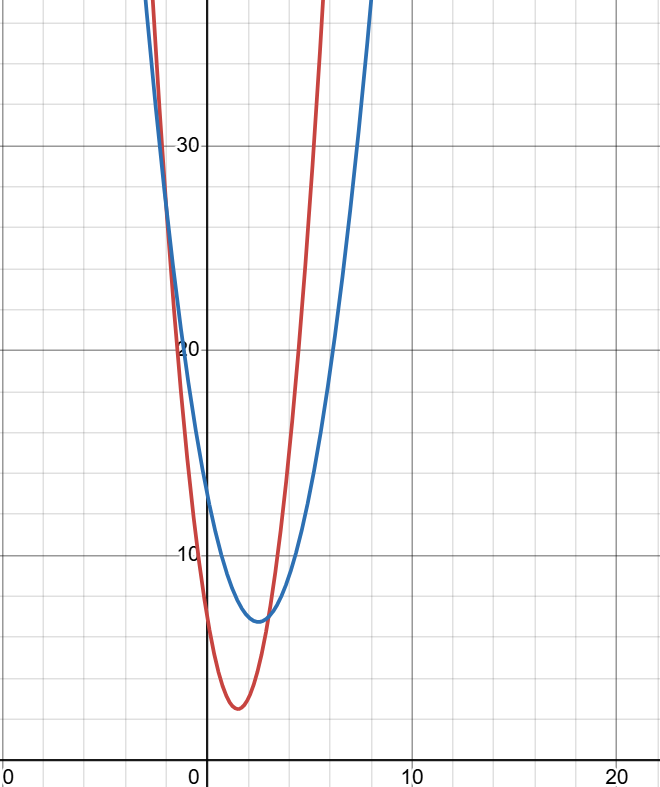
\includegraphics[width=0.7\linewidth]{5D-4.3-eryk.borczuch.INF.png}
    \caption{rood = y1 en blauw = y2}
\end{figure}


\begin{thebibliography}{999}
%\bibitem{a} Referentie
\end{thebibliography}
\end{document} 
